\section{$\beta$-$\gamma$ irradiator}
\label{sec:irradiador}
In order to carry out experiments with radiation,
we built an apparatus which allows us to expose samples to 
precise doses of $\beta$ and $\gamma$ rays,
while keeping the operator shielded.
The apparatus consists of a lead tube lined with PVC on its inner wall
(\figref{fig:corteirradiador}).
\fig{corteirradiador}{figuras/poster/corte.pdf}{Cutaway drawing of the irradiator}

All surfaces which might be exposed to $\beta$ particles are covered in PVC,
to stop the particles while producing the least possible amount of braking
X rays.

Near one end of the cavity is a \Strontium source
(\figref{fig:fuente})
\fig{fuente}{figuras/poster/fuente.pdf}{Cutaway drawing of the \Strontium $\beta$ source.}
in a plastic pocket attached to a rotating block of lead
(\figref{fig:piezagiratoria}).
\fig{piezagiratoria}{figuras/poster/piezagiratoria.png}
{Rotating assembly where the $\beta$ source is mounted.}
When the lead is interposed between the $\beta$ source and the inside of the cavity,
it is safe for people to open the cavity and handle the samples inside
(\figref{fig:posicionno}).
When the assembly is rotated towards the other side,
the $\beta$ source emits radiation into the cavity without any obstacles
(\figref{fig:posicionsi}).

The assembly was motorized by Javier Badía as part of his final annual laboratory course.
This allows for exposure to be controlled with a switch (or a computer program)
in a simple, fast and repeatable manner.
\begin{figure}[H]
    \centering
    \begin{subfigure}[b]{.45\textwidth}
        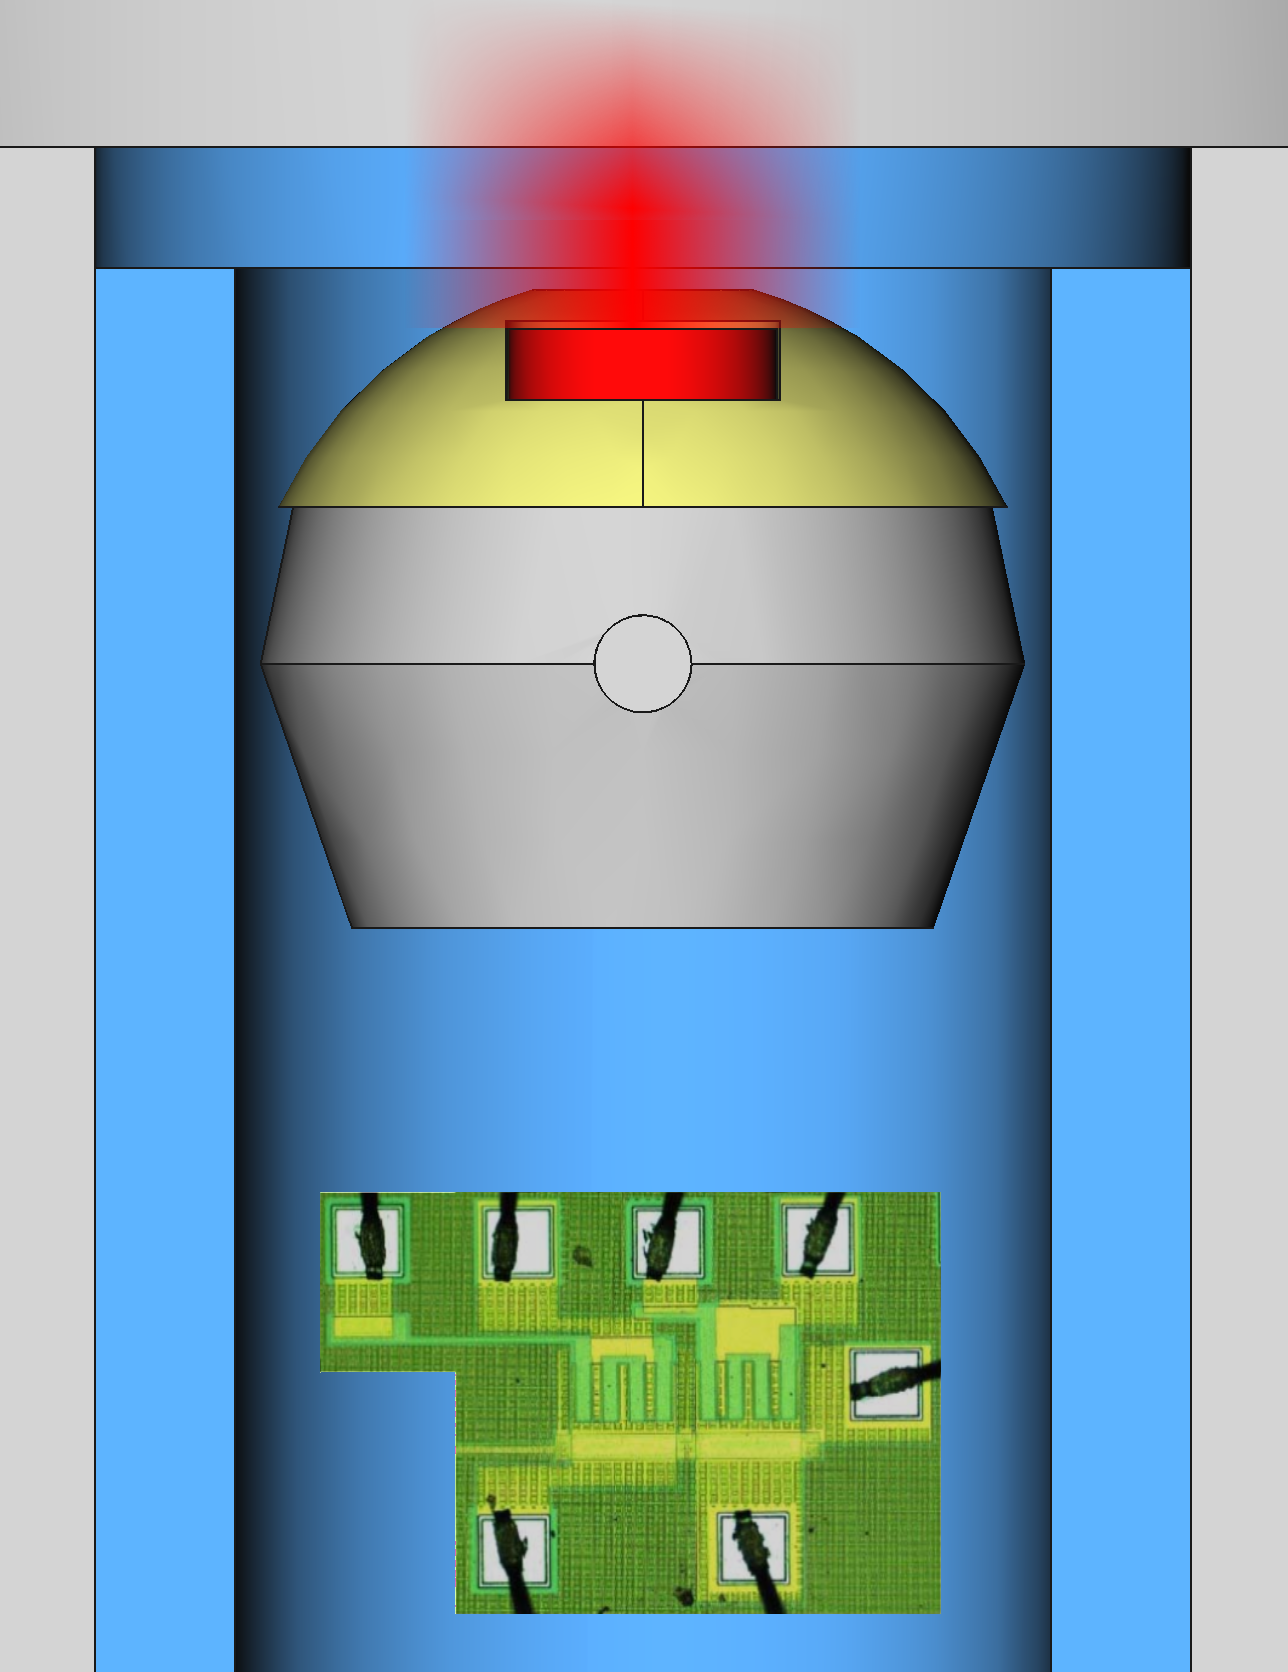
\includegraphics{figuras/poster/posicion_no.png}
        \caption{Safe position.}
        \label{fig:posicionno}
    \end{subfigure}
    \hspace{5mm}
    \begin{subfigure}[b]{.45\textwidth}
        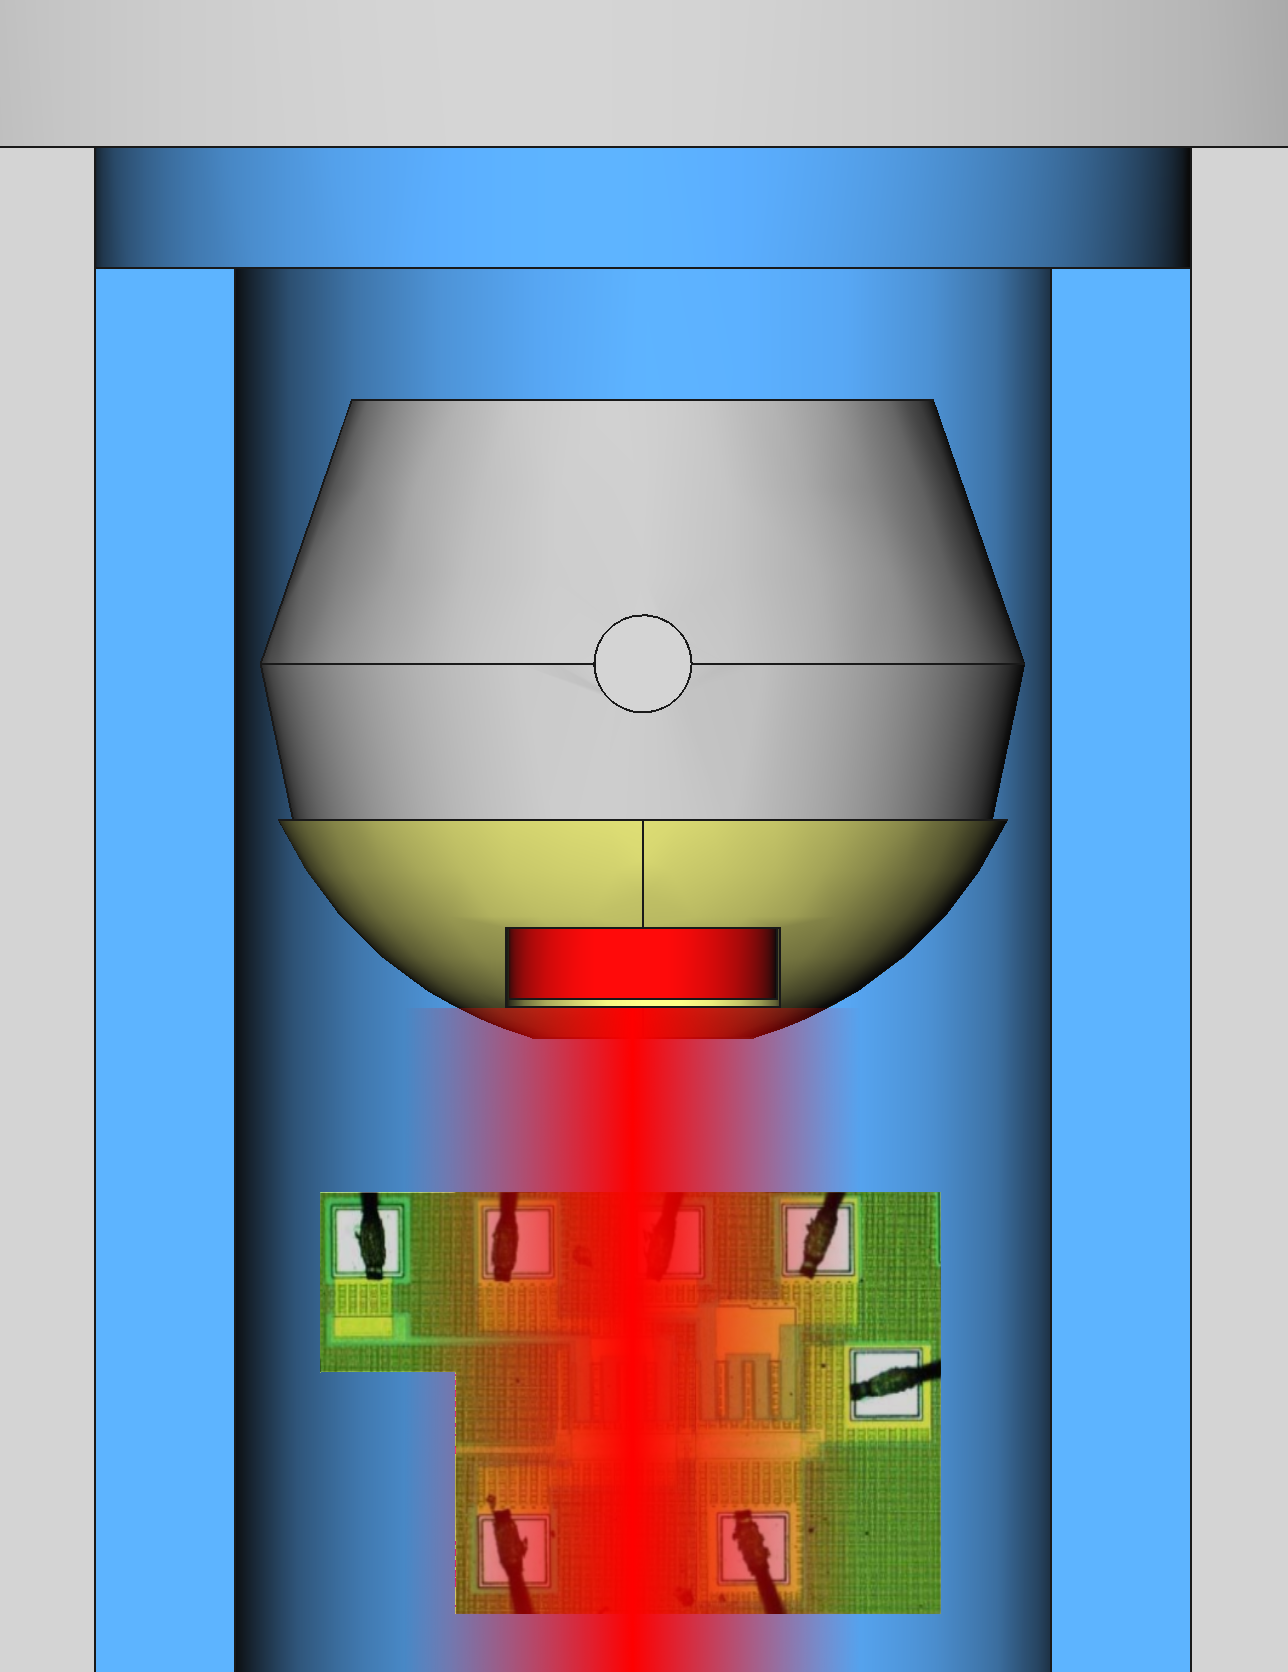
\includegraphics{figuras/poster/posicion_si.png}
        \caption{Irradiation position.}
        \label{fig:posicionsi}
    \end{subfigure}
    \caption{Rotating assembly positions.}
    \label{fig:posicionespieza}
\end{figure}
\subsection{Construction}
\subsubsection{Walls}
Both ends of the cavity were covered with 
\SI{10}{\milli\meter} thick, \SI{90}{\milli\meter} diameter acrylic disks.

For the sidewalls, we were not able to find \SI{10}{\milli\meter} thick PVC pipe.
Initially we considered molding tubes out of paraffin or acrylic.
In the end, we decided to use two concentric PVC pipes,
filling the gap between them with acrylic.
\subsubsection{Rotating assembly}
The rotating assembly is made out of cast lead which was turned on a lathe
(\figref{fig:construccion_mariposa}).
\fig{construccion_mariposa}{figuras/irradiador/construccion_mariposa.pdf}
{Construction steps for the rotating assembly.
The turning step required a handle for the chuck to hold.
This handle was cut after turning.}
For the casting step, we turned to Abraham Murillo, from the
Escuela Técnica Nº 33 Fundicion Maestranza del Plumerillo.
The shop turned a wooden pattern slightly bigger than the desired final dimensions.
This was due to
\begin{itemize}
    \item the thermal contraction of lead when it cools down, and
    \item the extra thickness necessary for the final turning step.
\end{itemize}
We packed sand around the pattern in order to create a mold.
We added a vent hole for the hot gases to escape,
and a tube for the liquid metal to flow into the mold
(\figref{fig:moldeplomo}).
\fig{moldeplomo}{figuras/irradiador/molde_plomo.pdf}
{Cross section of the mold used for the rotating lead piece.
It was built out of sand packed around a wooden pattern.
The liquid metal was poured in through the tube on the right.
The hole on top provides a vent for hot gases.}
The resulting cast has a rough surface due to the sand grains in the mold.
In order to give it the exact dimensions we required,
and a smooth finish,
we received assistance from 
Eriel Fernandez from the FIUBA machine shop.
While we originally planned for a spherical piece,
this was not feasible on a manual lathe.
Instead, we settled for a piecewise linear cross-section
which covers the irradiator cavity
and is able to rotate within it
(\figref{fig:torneo_simple}).
\fig{torneo_simple}{figuras/irradiador/torneo_simple.pdf}
{We chose a shape simple enough to turn in a manual lathe,
which covers the irradiator cavity and is able to rotate within it.
The last requirement is met by ensuring the corners are within a circle
whose diameter matches the cavity's inner diameter.}
The final dimensions are in \figref{fig:torneo}.
The softness of the material required careful turning at low RPM.
\fig{torneo}{figuras/irradiador/torneo.pdf}
{Cross section of the rotating lead piece after turning (all dimensions are in mm).}
\subsubsection{Pocket for radiation source}
The radiation source is held in a plastic pocket.
Although the source has a threaded hole which can be used to secure it,
screwing it in would require close manipulation
and exposing someone's hands to radiation for a length of time.
Therefore, we decided to use a pocket such that the source
can be quickly dropped in without lengthy exposures to radiation.

We aimed to stop all electrons before they reach the lead piece.
Therefore, we shaped the plastic as a spherical cap which covers
the lead as much as possible,
while still being able to rotate inside the cavity.

Due to the difficulty in resin-casting a rounded shape with a cavity,
we turned to Iván G. Pollitzer from the
Laboratorio Abierto de Electrónica at FIUBA.
Iván guided us in designing a 3D printed ABS piece.
It consists of two parts printed separately
(\figref{fig:blender}),
\fig{blender}{figuras/irradiador/blender_small.png}
{The two parts that we 3D printed in ABS and glued together.
The space between the two parts forms a pocket where the radiation source is held.}
which we then filled with acrylic and glued together.

We screwed the plastic to the lead piece using headless screws,
drilling and tapping holes in both pieces.
\subsection{Radiation protection calculations}
%
\subsubsection{Bremsstrahlung calculations}
The $\beta$ particles emitted from the radiation source are stopped in plastic,
where they produce braking radiation.
We calculate its magnitude starting from the energy spectrum of the emitted electrons.
Because the source is in secular equilibrium (equal \Strontium and \Yttrium activities),
we sum their spectra taken from
Radiological Toolbox\cite{eckerman2006radiological}
and then normalize to the source's nominal activity, \SI{100}{\milli\curie}
(\figref{fig:actividadsr90}).
\fig{actividadsr90}{figuras/irradiador/actividad.pdf}
{Electron energy spectrum for a
\Strontium source whose activity is \SI{100}{\milli\curie}\cite{eckerman_icrp_2007}.}
We then calculate the bremstrahlung spectrum by integrating \equref{eq:kramers}
(\figref{fig:espectrox}).
\fig{espectrox}{figuras/irradiador/espectrox.pdf}
{Calculated bremsstrahlung spectrum in the PVC outer wall.}
%
\subsubsection{X ray shielding in lead}
We applied \equref{eq:absorcionx} 
using lead absorption coefficients published by NIST\cite{xraycoef},
resulting in the attenuated spectrum in \figref{fig:xatenuado}.
\fig{xatenuado}{figuras/irradiador/xatenuado.pdf}
{Calculated X ray spectrum in the irradiator's outer face.}
% TODO: tasa de dosis final según distancia, comparar con mediciones
%
%
\subsubsection{Monte Carlo simulations with \Strontium source}
La fuente de \Strontium  emite electrones con un espectro amplio de
energías (\figref{fig:actividadsr90}).
Este consiste en la suma del espectro de emisión de \Strontium
y el de \Yttrium.
Simulamos un haz de electrones con este espectro incidiendo normalmente sobre
tejido blando, registrando la energía que depositan en función de la
profundidad (\figref{fig:deposicionsr90}).
\fig{deposicionsr90}{figuras/montecarlo/deposicion_sr90.pdf}
{Energía depositada en tejido blando en función de la distancia,
promediando entre electrones provenientes de una fuente de \Strontium.}
Así ajustamos una potencia de frenado de masa promedio $S/\rho$ (\figref{fig:stoppingsr90})
\fig{stoppingsr90}{figuras/montecarlo/stopping_sr90.pdf}
{Potencia de frenado promedio del tejido blando para electrones provenientes de
una fuente de \Strontium.
La cruz marca que a una profundidad de \SI{0.35}{\milli\meter} la tasa de dosis 
coincide con la tabulada en \cite{delacroix_radionuclide_2002}.}
que permite calcular tasa de dosis superficial mediante
\begin{align*}
    \dot D &= \frac{AS/\rho}{4\pi r^2}
\end{align*}
con $A=\SI{100}{\milli\curie}$ la actividad de la fuente.
La tasa de dosis calculada de este modo es comparable con la tabulada en
\cite{delacroix_radionuclide_2002} si se promedia hasta una profundidad de
\SI{.35}{\milli\meter}.
Esto sirve como verificación de que nuestras simulaciones Monte-Carlo producen
valores compatibles con los que se encuentran en la literatura.
\subsubsection{Cálculos Monte-Carlo del irradiador}
Buscamos una cota superior de la tasa de dosis fuera del irradiador.
Esto brinda la mayor confianza en que su operación no es peligrosa.
Ya que el espesor del plomo es de varias longitudes características de
atenuación ($1/\mu$),
sólo pasa una fracción muy pequeña de la radiación inicial.
Por lo tanto, hay que simular la emisión de 
muchos electrones de la fuente de \Strontium
para que llegue una cantidad apreciable de radiación a la cara exterior.
Así podemos estimar de forma precisa la tasa de dosis.

Una forma de reducir el tiempo de CPU necesario para simulaciones
es usar reducción de la varianza\cite{dressel_geometrical_2003}.
Esta es una técnica para cálculos Monte Carlo que introduce un sesgo en la
evolución de la partícula.
Por ejemplo, podemos aumentar la probabilidad de que una partícula atraviese
el plomo sin interactuar, en vez de scatterear.
Llevando la cuenta de cuan improbable es la historia de la partícula,
le damos un peso menor en la estadística final.
Esto concentra la simulación en darnos muchos eventos que nos interesan
(lo cual reduce la varianza de la estimación),
minimizando la capacidad de procesamiento necesaria.

Dada la dificultad de implementar reducción de la varianza en Geant4,
optamos por acelerar el cálculo simplificando la geometría.
Simulamos un irradiador con simetría esférica,
que consiste en un cascarón de \SI{10}{\milli\meter} de acrílico rodeado por
\SI{36}{\milli\meter} de plomo (\figref{fig:corte_esferico}). 
\fig{corte_esferico}{figuras/irradiador/corte_esfera.png}
{Corte de la geometría simplificada que se usó para simular el irradiador en
Geant4.}
Toda partícula en el irradiador tiene que atravesar al menos ese espesor de
acrílico y plomo.
Por lo tanto, la dosis real va a ser aún menor a la simulada.
Dada la simetría del problema, no tenemos en cuenta la distribución en
$\theta$ y $\phi$ sino que promediamos sobre ambas variables.
Esto reduce enormemente el número de eventos necesarios para una buena
estimación de la tasa de dosis.
El resultado se ve en la \figref{fig:dosis_irradiador}.
\fig{dosis_irradiador}{figuras/montecarlo/dosis_irradiador.pdf}
{Perfil de deposición de energía en la simulación Monte-Carlo del irradiador.}
La dosis en la cara exterior del irradiador es
de \SI{20.3}{\milli\sievert} por año.
Este valor es aceptable si se tiene en cuenta que,
en condiciones reales, se toca el irradiador durante intervalos muy cortos
y el resto del tiempo se está a distancias mucho mayores.
